\chapter{El LHC y el Experimento ATLAS} \label{chap:ch2}

\newthought{En este capítulo} presentaremos al experimento ATLAS, uno de los cuatro experimentos principales del LHC. Introduciremos inicialmente al complejo de aceleradores y los parámetros más importantes de un colisionador hadrónico. Luego, describiremos los distintos subdetectores de ATLAS y el sistema de trigger. Finalmente, desarrollaremos brevemente el procesamiento y distribución de los datos recolectados por el experimento.


\section{El Gran Colisionador de Hadrones}

El Gran Colisionador de Hadrones, o LHC (Large Hadron Collider) \cite{Brüning:782076} es un acelerador de hadrones superconductor de dos anillos, perteneciente a la Organización Europea para la Investigación Nuclear (CERN, por sus antiguas siglas en francés), ubicado en las afueras de la ciudad de Ginebra, Suiza. Posee una longitud de \SI{27}{km}, extendiéndose debajo de la frontera entre Francia y Suiza a una profundidad variable entre 50 y \SI{174}{m} de la superficie terrestre. El LHC ha sido construido en el mismo tunel en el que funcionó el acelerador $e^+ e^-$ LEP (Large Electron-Positron collider) \cite{Wyss1996} entre 1989 y 2000.

El LHC fue diseñado para colisionar protones a una energía de centro de masa\sidenote{Definimos la energía de centro de masa $\sqrt{s}$, como la cantidad total de energía del sistema protón-protón en el punto de interacción (IP, \textit{Interaction Point}), observado desde el sistema de laboratorio.} de $\sqrt{s} = \SI{14}{\TeV}$, e iones pesados con hasta \SI{2.76}{\TeV} por nucleón. El acelerador cuenta con cuatro puntos de interacción principales, donde se alojan los detectores más importantes: ATLAS~\cite{Aad2008}, CMS~\cite{Chatrchyan2008}, ALICE~\cite{Aamodt2008} y LHCb~\cite{AugustoAlves2008}, como podemos observar en la \cref{fig:ch2:lhc}.

\begin{figure}[t]
    \includegraphics[width=\linewidth]{Assets/Images/CERN_accelerators.pdf}
    \caption{Complejo de aceleradores del CERN \citeonly{Christiane:1260465}}
    \label{fig:ch2:lhc}
    \setfloatalignment{b}
\end{figure}

Para alcanzar las energías enunciadas, las partículas son aceleradas en múltiples etapas, a través de una cadena de pre-aceleradores. En el caso de los protones, con los que trataremos en este trabajo, el proceso comienza con la formación de paquetes de $\sim \num{1e11}$ protones, o \textit{bunches}, a partir de la ionización de átomos de hidrógeno y la separación electrostática de los electrones. Los \textit{bunches} de protones resultantes ingresan a un acelerador lineal de \SI{36}{\meter} de longitud (LINAC 2), donde adquieren una energía de \SI{50}{\MeV}. El paquete acelerado es transferido al \textit{Proton Synchroton Booster} (BOOSTER), el primer acelerador circular de la cadena, con \SI{160}{\meter} de circunferencia, alcanzando una energía de \SI{1.4}{\GeV}. El proceso continua en el \textit{Proton Synchroton} (PS), cuya circunferencia es de \SI{630}{\meter}, dejando a los protones con una energía de hasta \SI{25}{\GeV}. En el último paso antes de ingresar en el LHC, los protones incrementan su energía hasta \SI{450}{\GeV} en el \textit{Super Proton Synchroton} (SPS), que tiene \SI{7}{\kilo\meter} de circunferencia. Los paquetes de protones provenientes del SPS son inyectados en direcciones opuestas a los dos anillos del LHC, donde incrementarán su energía hasta la magnitud final $\sqrt{s}/2$.

\begin{marginfigure}
    \includegraphics[width=\linewidth]{Assets/Images/LHC_RF_cavities.jpg}
    \caption{Cavidad RF del LHC, donde se incrementa la energía de los \textit{bunches} de protones.}
    \label{fig:ch2:LHC_RF_cavities}
\end{marginfigure}

La aceleración de los bunches de protones en el LHC se realiza por medio de cavidades de radiofrecuencia (\cref{fig:ch2:LHC_RF_cavities}), con un gradiente del campo eléctrico máximo de \SI{5}{\mega\volt\per\meter} oscilando a \SI{400}{\mega\hertz}. Para mantener a los nucleones en una trayectoria aproximadamente circular\sidenote{Las cavidades de radiofrecuencia, al igual que los segmentos con imanes de enfoque cuadrupolares y las proximidades a los puntos de interacción son rectos; solo las secciones del LHC donde se encuentran los imanes dipolares son curvas.}, el LHC, cuenta con 1232 dipolos magnéticos superconductores, operando a \SI{1.9}{\kelvin} para generar campos magnéticos de hasta \SI{8.4}{\tesla}. Los dipolos están equipados con sextupolos, octupolos y decapolos, que permiten corregir las pequeñas imperfecciones de los campos magnéticos en las extremidades de los dipolos. Para mantener al haz enfocado y maximizar la probabilidad de una colisión, se emplean un conjunto de 392 imanes cuadrupolares superconductores, produciendo campos magnéticos de hasta \SI{6.8}{\tesla}. Los anillos del LHC conforman un entorno de ultra-alto vacío, con una presión máxima de \SI{1.3e-13}{\pascal}.

El diseño del LHC permite almacenar hasta 3564 bunches por anillo, aunque en la práctica este número se ve reducido a $n_b = 2808$. Con este número efectivo, los bunches se encuentran espaciados temporalmente en \SI{25}{\nano\second} ($f_{rev} = \SI{11}{\kilo\hertz}$), resultando en un cruce de haces en los cuatro puntos de interacción (\textit{bunch crossing}) con una frecuencia de $\sim\SI{40}{\mega\hertz}$. Junto a la energía de centro de masa de los nucleones $\sqrt{s}$, estas variables influyen directamente en la performance del acelerador, que podemos estudiar en términos del número de partículas por unidad de tiempo y área en los puntos de interación, denominada \textit{luminosidad instantánea}. Para colisiones protón-protón, este parámetro resulta
\[ \Lag = f_{rev} n_b \frac{N_1 N_2}{A} = f_{rev} n_b \frac{N_1 N_2 \gamma F}{4 \pi \epsilon_n \beta^*}, \]
donde $N_i$ es el número de partículas en cada bunch y $A = 4\pi\epsilon_n \beta^* / \gamma F$ es la sección efectiva del haz, definida en términos de la emitancia transversal normalizada\sidenote{Equivalente a la dispersión transversal media de las partículas del haz en el espacio de coordenadas e impulsos. Para el cálculo de la luminosidad final, $\epsilon_n$ es determinada experimentalmente, midiendo los perfiles transversales de los haces~\cite{Trad:2019liy}.} $\epsilon_n$, la función amplitud en el punto de interacción\sidenote{Este parámetro se encuentra relacionado al poder de focalización de los cuadrupolos. Se obtiene mediante simulaciones numéricas de los campos magnéticos.} $\beta^*$, el factor de Lorentz $\gamma = 1/\sqrt{1-v^2/c^2}$, y un factor de reducción geométrico $F$ debido al ángulo de cruce de los haces en el punto de interacción~\cite{Lee2019}. La luminosidad puede ser entendida como la magnitud que indica la capacidad de un acelerador de producir un determinado número de interacciónes de un dado proceso en el que se esté interesado, resultando en una tasa de eventos instantánea
\[ \dv{N}{t} = \sigma \Lag, \]
suponiendo una sección eficaz $\sigma$ del proceso de interés. Integrando en el tiempo obtenemos el número total de eventos $N$ a medirse en un dado tiempo $t$, definiendo entonces la luminosidad integrada como
\[ L = \frac{N}{\sigma} = \int_0^t \Lag(t') \dd{t'}, \]
expresada usualmente en unidades de $\si{\femto\barn^{-1}} = \SI{1e-39}{\centi\meter^{-2}}$. En el período de operación del LHC 2015-2018, conocido como \textit{Run 2}, se alcanzó una energía máxima de $\sqrt{s} = \SI{13}{\TeV}$ (correspondiente a \SI{6.5}{\TeV} por nucleón, con una velocidad de $0.99999999c$) y una luminosidad instantánea media de \SI{1.4e-5}{\femto\barn^{-1} \second^{-1}}. La \cref{fig:ch2:lhc_atlas_luminosity} representa la luminosidad integrada como función del tiempo de recolección de datos del LHC, y la luminosidad integrada de las colisiones medidas y procesadas por el experimento ATLAS, que será descrito en la siguiente sección.

\begin{marginfigure}
    \includegraphics[width=\linewidth]{Assets/Plots/Lumi_ATLAS.pdf}
    \caption{Luminosidad integrada entregada, capturada por ATLAS y calificada para estudiar física durante el Run 2.}
    \label{fig:ch2:lhc_atlas_luminosity}
\end{marginfigure}

Actualmente, el LHC se encuentra en preparativos para comenzar el tercer período de toma de datos (Run 3), iniciando en mediados de 2022 hasta fines de 2025, luego de transitar un período no-operativo que comenzó en 2019 (\textit{long shutdown 2}), al finalizar el Run 2. Durante los períodos no-operativos se realizaron tareas de mantenimiento y mejoras del LHC y los detectores, preparando el complejo de aceleradores y los experimentos para la siguiente etapa del LHC, el HL-LHC (\textit{High Luminosity LHC}), donde se incrementará la luminosidad.





\section{El Experimento ATLAS}

ATLAS (\textit{A Toroidal Lhc AparatuS}) es uno de los dos experimentos multipropósito del LHC, diseñado para estudiar las partículas producidas en colisiones protón-protón (\textit{pp}) y en colisiones de iones pesados a las altas energías provistas por el LHC. 

El detector de ATLAS~\cite{Aad2008} posee una geometría aproximadamente cilíndrica, alcanzando una cobertura de casi $4\pi$ alrededor del punto de interacción, como podemos observar en la \cref{fig:ch2:atlas_schematic}. Se divide geométricamente en dos regiones: la parte central denominada \textit{barrel}, y las regiones extremas donde se hubican los \textit{endcaps} (``tapas externas''). En la región \textit{barrel}, los detectores se ubican en forma de cilindros concéntricos rodeando al eje del haz, mientras que en las regiones de los \textit{endcaps} se disponen como discos perpendiculares a la dirección del haz. 

\begin{figure*}[t]
    \centering
    \includegraphics[width=0.99\linewidth]{Assets/Images/ATLAS_schematic.jpg}
    \caption[][-2em]{Esquema general del detector de ATLAS.}
    \label{fig:ch2:atlas_schematic}
\end{figure*}

ATLAS cuenta con múltiples sub-detectores, cada uno especializado en medir las propiedades cinemáticas de las distintas partículas presentes en el estado final del proceso, como se exhibe en la \cref{fig:ch2:atlas_interactions}. En la región más interna alrededor del punto de interacción se encuentra el detector interno de trazas (ID, \textit{Inner Detector}), inmerso en un campo magnético solenoidal de \SI{2}{\tesla} (producido por un solenoide superconductor que envuelve inmediatamente al ID), necesario para curvar la trayectoria de las partículas cargadas y así medir su impulso. El ID provee una precisa reconstrucción de las trazas de las partículas cargadas, con una alta granularidad.

\begin{marginfigure}[-70pt]
    \centering
    \includegraphics[width=0.99\marginparwidth]{Assets/Images/ATLAS_interactions.pdf}
    \caption{Corte transversal esquemático del detector ATLAS. Se muestran las interacciones de distintos tipos de partículas con los sub-detectores; de izquierda a derecha: muón, fotón, protón, neutrón, electrón y neutrino. Las trayectorias punteadas son invisibles al detector.}
    \label{fig:ch2:atlas_interactions}
\end{marginfigure}

Rodeando al ID encontramos un sistema de calorímetros de dos componentes: un calorímetro electromagnético (ECAL, \textit{Electromagnetic CALorimeter}), diseñado para medir principalmente la energía depositada por fotones y electrones; y un calorímetro hadrónico (HCAL, \textit{Hadronic CALorimeter}) exterior, midiendo la energía de los jets y hadrones producidos en la colisión y posteriores interacciones.

Finalmente, en la capa más externa de ATLAS, encontramos el espectrómetro de muones (MS, \textit{Muon Spectrometer}), donde tres sistemas de imanes toroidales intercalados proveen campos magnéticos con un gradiente entre \num{2} y \SI{6}{\tesla\meter}, utilizados para curvar la trayectoria de los muones y así determinar su momento y energía.

Las dimensiones resultantes de esta geometría y composición transforman a ATLAS en el detector de partículas más grande construído hasta el momento, con \SI{44}{\meter} de largo y \SI{25}{\meter} de diámetro, superando las \num{7000} toneladas.




\subsection{Sistema de coordenadas} \label{sec:ch2:atlas_coordinates}

ATLAS adopta un sistema de coordenadas cartesiano con origen en el IP en el centro del detector, colocando el eje $z$ a lo largo del haz, con valores crecientes de $x$ en la dirección del centro del LHC y valores crecientes de $y$ hacia arriba. El álgulo azimutal $\phi$ es medido alrededor del eje del haz, en el plano transversal $x$-$y$, mientras que el ángulo polar $\theta$ es medido con respecto al eje del longitudinal del haz. La disposición de los ejes puede ser observada en la \cref{fig:ch2:atlas_coordinates}

\begin{marginfigure}
    \includegraphics[width=\linewidth]{Assets/Images/ATLAS_coordinates.pdf}
    \caption{Sistema de coordenadas de ATLAS}
    \label{fig:ch2:atlas_coordinates}
\end{marginfigure}

En el contexto de un acelerador, donde esperamos que la totalidad del impulso de las partículas se encuentre en la dirección del haz, definimos la rapidez $y$ a partir de la energía total de la partícula y la componente longitudinal del momento como
\[ y = \inv{2} \log(\frac{E + p_z}{E - p_z}). \]
En el límite ultra-relativista, donde la relación de dispersión puede ser aproximada como $E^2 = m^2 + p^2 \approx p^2$, esta cantidad se aproxima para partículas masivas (y vale de manera exacta para partículas no-masivas) a la pseudorapidez $\eta$, que se puede expresar directamente en términos del ángulo respecto al haz $\theta$ como
\[ \eta = \inv{2} \log(\frac{p + p_z}{p - p_z}) = -\log\qty[ \tan(\frac{\theta}{2})]. \]
La \cref{fig:ch2:pseudorapidity} contiene una comparación geométrica entre los valores de la coordenada $\theta$ y su valor correspondiente de $\eta$.
\begin{marginfigure}
    \includegraphics[width=\linewidth]{Assets/Images/Pseudorapidity.pdf}
    \caption{Representación geométrica de la relación entre el ángulo polar $\theta$ y la pseudorapidez $\eta$. La región de $\eta$ grande ($\theta$ pequeño) recibe el nombre de \textit{forward}.}
    \label{fig:ch2:pseudorapidity}
\end{marginfigure}
En física de altas energías, esta nueva variable es preferida sobre el ángulo polar $\theta$, ya que la multiplicidad de las partículas producidas resulta aproximadamente constante como función de $\eta$, y la diferencia de pseudorapidez entre dos partículas es invariante frente a boosts de Lorentz en la dirección del haz. Junto con el ángulo azimutal $\phi$, también invariante ante boosts en la dirección privilegiada, nos permite definir una medida de distancia angular entre partículas
\[ \Delta R = \sqrt{\Delta\eta^2 + \Delta\phi^2}, \]
que será de vital importancia en los próximos capítulos.

Debido a que los protones inciden en la dirección longitudinal $z$, es razonable suponer que el momento transverso de los partones es aproximadamente nulo. El momento transverso total $p_T = \sqrt{p_x^2 + p_y^2}$ es conservado durante la colisión. Resulta útil definir también la energía transversa
\[ E_T = \frac{E}{\cosh\eta}, \]
donde $E$ es la energía total de la partícula. Si bien $E_T$ no es una cantidad conservada, para partículas muy energéticas de masa pequeña, la corrección es menor\sidenote[][-11em]{%
Expandiendo en $m/p_T$, 
\begin{align*} 
    \frac{E_T}{p_T} = \frac{E}{p} &= \sqrt{1 + \frac{m^2}{p^2}} \\
                                  &= \sqrt{2 + \sin^2(\theta) \frac{m^2}{p_T^2}} \\
                                  &\approx 1 + \inv{2} \sin^2\theta \frac{m^2}{p_T^2}.
\end{align*}
}~\cite{gallicchio2018quit}. En la dirección longitudinal, la fracción de momento del protón adquirida por cada uno de los partones interactuantes es desconocida: parte del impulso es transferido en la interacción dura, mientras que cierta fracción remanente escapa al detector a lo largo del haz. Por lo tanto, no es posible reconstruir el movimiento longitudinal del centro de masa en la interacción, haciendo imposible aplicar las leyes de conservación sobre la cinemática longitudinal (y, por extensión, total) de cada evento.


\subsection{Subsistemas}

Procederemos a describir brevemente los subsistemas principales de ATLAS. Para una información más detallada, el lector puede dirigirse al informe técnico de la colaboración \cite{Aad2008}.

\subsubsection{Sistema de Imanes}

El sistema de imanes de ATLAS permite una precisa medición del momento de las partículas cargadas, y de la identificación de la propia carga \cite{TenKate1999}. Está compuesto por tres conjuntos de imanes superconductores, como podemos observar en la \cref{fig:ch2:atlas_magnets}: un Solenoide Central, un toroide en la región de \textit{barrel} y dos toroides más pequeños en las regiones de los \textit{endcaps}.

Rodeando al ID se encuentra el Solenoide Central, proveyendo un campo magnético de \SI{2}{\tesla} en solo \SI{4.5}{\centi\meter} de espesor, utilizado para reconstruir el momento transverso de las partículas cargadas.

Los imanes toroidales permiten la reconstrucción del momento de los muones en el MS. El toroide de la región \textit{barrel} se encuentra compuesto por 8 bobinas, encerrando una masiva región de \SI{26}{\meter} de largo y \SI{20}{\meter} de diámetro. Este produce una intensidad de campo media de \SI{0.5}{\tesla}, con máximos de \SI{3.5}{\tesla}. Los dos toroides de los \textit{endcaps} se encuentran encerrados en criostatos de \SI{11}{\meter} de diámetro. Están también formados por 8 bobinas superconductoras, produciendo campos de hasta \SI{4}{\tesla}, con una intensidad media de \SI{1}{\tesla}.

Los imanes se encuentran refrigerados por un sistema cerrado de helio líquido, mantenido a \SI{4.5}{\kelvin}.

\begin{marginfigure}
    \includegraphics[width=\linewidth]{Assets/Images/ATLAS_magnets.pdf}
    \caption{Esquema del sistema de imanes de ATLAS.}
    \label{fig:ch2:atlas_magnets}
\end{marginfigure}

\subsubsection{Detector Interno}

El detector interno cuyo esquema general se exhibe en la \cref{fig:ch2:atlas_ID}, es el más próximo al haz, combinando detectores de muy alta resolución (cerca del punto de interación) con detectores contínuos de trazas. Se encuentra inmerso en el campo magnético de \SI{2}{\tesla} producido por el solenoide central del sistema de imanes. Es capaz de determinar el momento trasverso con una resolución relativa de
\[ \frac{\sigma_{p_T}}{p_T} = 0.05\% \cdot p_T \oplus 1\%, \]
y cuenta con una resolución en la posición de los vértices de hasta aproximadamente \SI{20}{\micro\meter} en el plano transverso (en las direcciones$x$ e $y$) y \SI{50}{\micro\meter} en la dirección $z$~\cite[-2em][]{ATL-PHYS-PUB-2015-026}. Describiremos brevemente a continuación sus sub-sistemas.

\begin{figure*}[t]
    \centering
    \subfloat[][\label{fig:ch2:atlas_ID:cut}]{\includegraphics[width=0.55\fulllinewidth]{Assets/Images/ATLAS_ID_cut.jpg}}
    \subfloat[][\label{fig:ch2:atlas_ID:layers}]{\includegraphics[width=0.45\fulllinewidth]{Assets/Images/ATLAS_ID_layers.jpg}}
    \caption{Detector interno de ATLAS: esquema general \subref{fig:ch2:atlas_ID:cut}; capas del detector atravesadas por una partícula cargada de $p_T = \SI{10}{\GeV}$ \subref{fig:ch2:atlas_ID:layers}.}
    \label{fig:ch2:atlas_ID}
\end{figure*}

%\begin{marginfigure}
%    \noindent\subfloat[\label{fig:ch2:atlas_ID:cut}]{\includegraphics[width=\marginparwidth]{Assets/Images/ATLAS_ID_cut.jpg}}\\
%    \noindent\subfloat[\label{fig:ch2:atlas_ID:layers}]{\includegraphics[width=\marginparwidth]{Assets/Images/ATLAS_ID_layers.jpg}}
%
%    \caption{Detector interno de ATLAS: esquema general \subref{fig:ch2:atlas_ID:cut}; capas del detector atravesadas por una partícula cargada de $p_T = \SI{10}{\GeV}$ \subref{fig:ch2:atlas_ID:layers}.}
%    \label{fig:ch2:atlas_ID}
%\end{marginfigure}

\paragraph{Detector de Píxeles}

El detector de píxeles fue construido para medir la posición de las trazas de partículas cargadas con la más alta precisión posible, y es vital para la reconstrucción de los vértices primarios y secundarios de la reacción. Se compone de cuatro capas.

A solo \SI{0.2}{\milli\meter} de la tubería de $\textrm{Be}$ por la que circula el haz se encuentra la \textit{Insertable B-Layer} (IBL), compuesta por 8 millones de sensores de silicio de lectura rápida, que detectan el paso de partículas cargadas mediante la deposición de carga inducida. El tamaño de los píxeles es de $50 \times \SI{50}{\micro\meter^2}$, con una resolución combinada de \SI{8}{\micro\meter} en el plano transverso y \SI{40}{\micro\meter} en $z$. Esta capa contribuye a mejorar la eficiencia en la identificación de trazas, vértices, y en la identificación de bottom quarks, que decaen típicamente fuera del radio del IBL (este se encuentra a \SI{3.5}{\centi\meter} del IP dentro del tubo).

Las siguientes tres capas se encuentran dispuestas en forma de cilíndros concéntricos en la región \textit{barrel} (a \SI{17}{\milli\meter} de la IBL), cubriendo la región $\abs{\eta} < 1.9$, y en forma de discos perpendiculares al eje del haz en los \textit{endcaps}, extendiendo la cobertura hasta $\abs{\eta} < 2.5$. Su principio de funcionamiento es, al igual que en la IBL, la detección de partículas cargadas mediante la medida de la deposición de la carga inducida en una capa de silicio por ionización. El sistema contiene en total 80 millones de sensores, cada uno con una resolución de \SI{10}{\micro\meter} en el plano transverso y \SI{115}{\micro\meter} en el eje $z$.

\paragraph{Detector Semiconductor de Trazas (SCT)}

Rodeando al detector de píxeles se encuentran las cuatro capas de módulos de sensores del SCT en la región \textit{barrel} y los nueve discos transversales al eje del haz en los \textit{endcaps}. El SCT está diseñado para medir las trazas con alta precisión en la zona intermedia del detector, cubriendo el rango $\abs{\eta} < 2.5$. Está formado por sensores de silicio segmentados en micro-bandas, con una resolución espacial de \SI{17}{\micro\meter} en el plano transverso y \SI{580}{\micro\meter} en $z$. La segmentación más gruesa, comparada con la del Detector de Píxeles, es posible en este caso al esperar una menor multiplicidad de partículas en esta región. Esto permite la reducción de costos y de canales de lectura.

\paragraph{Detector de Radiación de Transición (TRT)}

El TRT es el subsistema más externo del ID, habiendo sido diseñado no solo para detectar partículas cargadas, sino también para distinguir entre partículas pesadas y livianas. El TRT se compone de \textit{drift tubes} (tubos de deriva) de \SI{4}{\milli\meter} de diámetro, con un gas\sidenote{Una mezcla gaseosa de 70\% de $\textrm{Xe}$, 27\% de $\textrm{CO}_2$ y 3\% de $\textrm{O}_2$.} que se ioniza al ser atravesado por partículas cargadas y se detecta la radiación de transición. Los electrones producidos son colectados por un ánodo, pudiendo relacionar el tiempo de deriva con una medida de la distancia hasta la traza de la partícula incidente con una resolución de \SI{130}{\micro\meter}. Además, los tubos se encuentran cubiertos de fibras de polipropileno con un índice de refracción diferente, por lo que las partículas que atraviesan el detector emiten radiación con una intensidad proporcional a $\gamma = E/m$. De esta forma, el TRT permite distinguir partículas cargadas pesadas como $\pi^\pm$ y $K^\pm$ de aquellas más livianas, como $e^\pm$. La región \textit{barrel} contiene 50000 tubos paralelos al eje del haz, y en la región de los \textit{endcaps} cuentan con 320000 tubos orientados radialmente, abarcando un rango total de $\abs{\eta} < 2.0$. Su resolución espacial es de \SI{170}{\micro\meter}.



\subsubsection{Calorímetros} \label{sec:ch2:atlas:calo}

\begin{marginfigure}
    \subfloat[][\label{fig:ch2:atlas_calorimeters:all}]{\includegraphics[width=\marginparwidth]{Assets/Images/ATLAS_Calorimeters.pdf}}\\
    \subfloat[][\label{fig:ch2:atlas_calorimeters:endcaps}]{\includegraphics[width=\marginparwidth]{Assets/Images/ATLAS_Calorimeters_endcaps.pdf}}
    \caption{Sistema de calorímetros de ATLAS: esquema general \subref{fig:ch2:atlas_calorimeters:all}; calorímetros de las regiones de los \textit{endcaps}, donde la parte más próxima al IP se encuentra a la izquierda de la imágen \subref{fig:ch2:atlas_calorimeters:endcaps}.}
    \label{fig:ch2:atlas_calorimeters}
\end{marginfigure}

El sistema de calorímetros de ATLAS está formado por una componente electromagnética (ECAL) y una hadrónica (HCAL), y está diseñado para medir la energía y la posición de las partículas incidentes, mediante la absorción de la energía depositada por las cascadas de partículas secundarias generadas en el material por las partículas producidas en la colisión (\cref{fig:ch2:atlas_calorimeters}). Haciendo uso de sus dos componentes, permite discriminar a los electrones y fotones de los hadrones (jets) producidos. Este sistema provee una cobertura casi hermética alrededor del IP, de $\abs{\eta} < 4.9$ y completa en $\phi$, permitiendo medir el desbalance energético. Posee una granularidad más fina en la región  \textit{barrel} de $\eta$ que coincide con el ID. Además, provee la información utilizada por el sistema de L1-Trigger.

Este subsistema posee una resolución de la energía de las partículas incidentes dada por
\[ \frac{\sigma_E}{E} = \frac{a}{\sqrt{E}} \oplus b \oplus \frac{c}{E}, \]
con $a$, $b$ y $c$ constantes, donde el primer término está relacionado con las fluctuaciones del desarrollo de las cascadas, el término constante $b$ tiene en cuenta las inhomogeneidades del detector y el último término está asociado con el ruido electrónico. El valor de los coeficientes depende de los objetos incidentes (al presentar distintas interacciones debido a su naturaleza): para $e^\pm$ en el ECAL se tiene $a \sim 10\% \ \si{\GeV^{1/2}}$ y $b \sim 5\%$, mientras que para $\pi^\pm$ en el centro del detector se tiene $a \sim 50\% \ \si{\GeV^{1/2}}$ y $b \sim 5\%$ \cites[-4.5em][]{Spettel2016}[-1.5em][]{Plucinski2014}.

\paragraph{Calorímetro Electromagnético (ECAL)}

El ECAL es un calorímetro de muestreo inhomogéneo no compensado, que utiliza $\textrm{Pb}$ como material absorbente en una geometría de acordeón, y $\textrm{LAr}$ ($\textrm{Ar}$ líquido, refrigerado a \SI{89}{\kelvin}) como medio activo. Las partículas incidentes interactuan con las placas de $\textrm{Pb}$, creando una cascada de partículas cargadas y neutras. Las partículas cargadas ionizan el $\textrm{LAr}$ que se encuentra entre las placas, y los electrones liberados son colectados por un electrodo central de Kapton/$\textrm{Cu}$, sometidos a un campo eléctrico. La señal total en el medio activo resulta proporcional a la energía total de la partícula incidente.

El calorímetro está dividido en dos mitades dentro de la región \textit{barrel} ($\abs{\eta} < 1.475$, con una división en $\eta = 0$), y en dos componentes en los \textit{endcaps} ($1.375 < \abs{\eta} < 3.2$) conocidos como EMEC (\textit{ElectroMagnetic Endcap Calorimeter}). La región de transición entre el \textit{barrel} y los \textit{endcaps}, conocida como \textit{crack}, no cuenta con detectores, ya que allí se alojan las conexiones del sistema. Se suele requerir, por lo tanto, que los electrones y fotones utilizados en el análisis estén fuera de esta. La región de \textit{barrel} cuenta con 110000 canales de medición, mientras que los \textit{endcaps} solo poseen 1024 canales cada uno.

\begin{marginfigure}[-12em]
    \centering
    \subfloat[][\label{fig:ch2:atlas_calorimeters:ECAL:material:barrel}]{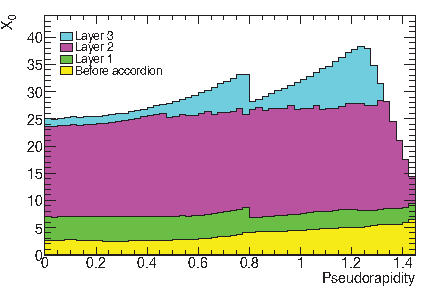
\includegraphics[width=0.99\marginparwidth]{Assets/Plots/ECAL_barrel_material.pdf}}\\
    \subfloat[][\label{fig:ch2:atlas_calorimeters:ECAL:material:endcaps}]{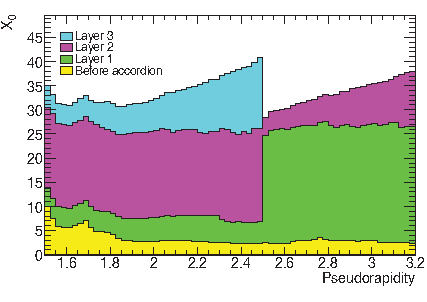
\includegraphics[width=0.99\marginparwidth]{Assets/Plots/ECAL_endcaps_material.pdf}}
    \caption{Cantidad de material acumulado en las distintas capas del ECAL en unidades de longitud de radiación $X_0$, en función de $\abs{\eta}$. Región \textit{barrel} \subref{fig:ch2:atlas_calorimeters:ECAL:material:barrel} y \textit{end-caps} \subref{fig:ch2:atlas_calorimeters:ECAL:material:endcaps}.}
    \label{fig:ch2:atlas_calorimeters:material}
\end{marginfigure}

En la región diseñada para medidas de precisión ($\abs{\eta} < 2.5$, excluyendo el crack), el ECAL está segmentado en tres capas concéntricas al eje principal de ATLAS. La primera capa se encuentra formada por bandas de fina granularidad en $\eta$, para discriminar entre fotones aislados y pares de fotones espacialmente cercanos provenientes del decaimiento de mesones neutros (como $\pi^0$). Los electrones y fotones con alto $E_T$ entregan la mayor parte de su energía en la segunda capa, con una granularidad lateral de $0.025 \times 0.025$ en el plano $\eta$-$\phi$. La tercer capa, de menor granularidad, absorbe la energía depositada en las colas de la lluvia.

En la región \textit{barrel}, el espesor del ECAL es mayor a 22 longitudes de radiación\sidenote{Definimos una longitud de radiación $X_0$ como la distancia media sobre la cual la energía de un electrón se reduce a $1/e$ de su energía inicial. Para los fotones, una reducción similar se obtiene a $9/7 X_0$.} ($X_0$), y mayor a $24 X_0$ en los \textit{endcaps}, como podemos observar en la \cref{fig:ch2:atlas_calorimeters:material}. Casi la totalidad de la energía electromagnética de partículas livianas y no-masivas, como $e^\pm$ y $\gamma$, resulta absorbida en el ECAL. En partículas cargadas más masivas, como hadrones, una parte de la energía es depositada en el ECAL antes de llegar al HCAL.

\paragraph{Calorímetro Hadrónico (HCAL)}

El HCAL, compuesto por tres subsistemas, es responsable de medir la energía de los hadrones neutros y cargados masivos, brindando una discriminación adicional para electrones. Este detector se extiende hasta $\abs{\eta} < 4.9$, permitiendo cubrir prácticamente la totalidad de los $4\pi$ desde el IP.

\begin{marginfigure}[5em]
    \centering
    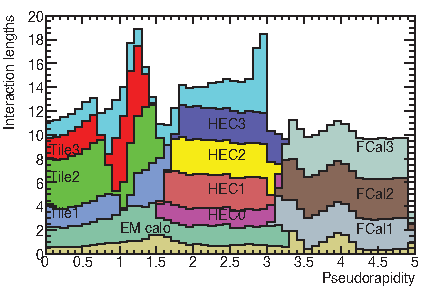
\includegraphics[width=0.99\marginparwidth]{Assets/Plots/HCAL_material.pdf}
    \caption{Cantidad de material acumulado en las distintas capas del HCAL, en unidades de longitud de interacción $\lambda$, en función de $\abs{\eta}$.}
    \label{fig:ch2:atlas_calorimeters:HCAL:material}
\end{marginfigure}

En la región \textit{barrel} ($\abs{\eta} < 1.7$), se ubica el \textit{Tile Calorimeter}, un calorímetro de muestreo que utiliza placas de acero como material absorbente y 420000 tejas centelladoras plásticas intercaladas como material activo, conectadas por medio de fibras ópticas a un conjunto de 9500 tubos fotomultiplicadores. Se encuentra dividido en dos partes: $\abs{\eta} < 1.0$ y $0.8 < \abs{\eta} < 1.7$, extendiéndose en radio entre \SI{2.28}{\meter} a los \SI{4.25}{\meter}. Posee una granularidad de $0.1\times0.1$ en el plano $\eta$-$\phi$.

En la región de los \textit{endcaps} ($1.5 < \abs{\eta} < 3.2$, con un diámetro exterior de \SI{4.6}{\meter}), se encuentra un calorímetro hadrónico de muestreo (HEC, \textit{Hadronic Endcap Calorimeter}), con $\textrm{LAr}$ como medio activo y placas de $\textrm{Cu}$ como absorbente, dispuestas perpendicularmente al haz.

El \textit{Forward Calorimeter} (FCal), ubicado a cada lado a \SI{4.7}{\meter} del IP, extiende la cobertura del sistema a $\abs{\eta} < 4.9$. El FCal emplea también $\textrm{LAr}$ como medio activo y $\textrm{Cu}$ o $\textrm{W}$ como material absorbente. Este último calorímetro de muestreo posee una granularidad de $0.2\times0.2$ en el plano $\eta$-$\phi$, y se utiza principalmente para el cálculo de la energía transversa faltante ($E_T^{miss}$) y en la reconstrucción de jets en regiones muy cercanas al eje del haz.

En total, el HCAL posee un espesor mayor a 7.7 longitudes de interacción hadrónica\sidenote{Similar a $X_0$, definimos la longitud de interacción hadrónica $\lambda$ como la distancia media sobre la cual la energía de un hadrón se reduce a $1/e$ de su energía inicial.} ($\lambda$) en la región \textit{barrel}, como se muestra en la \cref{fig:ch2:atlas_calorimeters:HCAL:material}\sidenote{Si se consideran las pérdidas de energía por interacción con el ECAL, este valor asciende a $9.7\lambda$.}, por lo que toda la energía de los hadrones que ingresan al HCAL queda depositada en el detector.

\subsubsection{Espectrómetro de Muones}

El Espectrómetro de muones (MS, \textit{Muon Spectrometer}) es el subsistema de detectores más externo de ATLAS, con la tarea de detectar y medir la posición y momento de los muones de alto $p_T$ producidos en la interacción y brindar rápida información al sistema de Trigger sobre la identificación de muones. Estas son las únicas partículas que alcanzan el MS, habiéndose depositado en su totalidad la energía de las otras partículas detectables en el ID, el ECAL y el HCAL. El MS cuenta con 4000 cámaras de detección de muones, utilizando distintas tecnologías. En su interior también se encuentran las bobinas superconductoras de los imanes toroidales del experimento, como se puede observar en la \cref{fig:ch2:atlas_MS}.

\begin{figure}[t]
    \centering
    \includegraphics[width=0.8\linewidth]{Assets/Images/ATLAS_MS.pdf}
    \caption{Espectrómetro de muones de ATLAS.}
    \label{fig:ch2:atlas_MS}
    \setfloatalignment{b}
\end{figure}

Las cámaras para medidas de precisión, llamadas \textit{Monitored Drift Tubes} (MDT) cubren el rango de $\abs{\eta} < 2.7$. Estas miden la curvatura de las trayectorias de los muones bajo el mismo principio de funcionamiento que el TRT: son tubos presurizados, donde el gas en su interior se ioniza ante el paso de una partícula, pudiendo relacionar el tiempo de deriva de los electrones producidos hasta ser colectados por el ánodo central con la distancia de la traza. El MDT posee 1171 cámaras de detección, con un total de 354240 tubos de \SI{3}{\centi\meter} de diámetro, alcanzando una resolución espacial de \SI{80}{\micro\meter}.

En los \textit{endcaps}, con $\abs{\eta} > 2.0$, frente a los dos toroides laterales, se encuentran las \textit{Cathode Strip Chambers} (CSC), con 70000 canales de adquisición. Estos sub-detectores cuentan con una alta resolución espacial (\SI{60}{\micro\meter}), midiendo la carga depositada en un ánodo, producto de una cascada de electrones generada en su entorno.

Los dos sistemas remanentes, con menor granularidad pero mayor velocidad, están principalmente orientados a proveer información rápida al sistema de L1-Trigger. En la sección \textit{barrel}, con $\abs{\eta} < 1.05$, las \textit{Resistive Plate Chambers} (RPC) proveen una estimación rápida del momento de los muones. Las RPCs miden la descarga ocasionada entre dos placas resistivas paralelas sometidas a una alta diferencia de potencial (\SI{5000}{\volt/\milli\meter}), tras la ionización del volumen de gas interno causada por el paso de muones energéticos. Finalmente, en la región \textit{endcap}, con $\abs{\eta} < 2.4$, se encuentran las \textit{Thin Gap Chambers} (TGC), con un propósito y funcionamiento análogo a las CSCs.



\subsection{Sistema de Trigger} \label{sec:ch2:atlas:trigger}

\begin{marginfigure}[-50em]
    \includegraphics[width=0.99\marginparwidth]{Assets/Plots/mu_2015_2018.pdf}
    \caption{Distribuciones del número de interacciones por \textit{bunch crossing} (\textit{pileup}) durante el Run 2.}
    \label{fig:ch2:lhc_atlas_pileup}
\end{marginfigure}

\begin{marginfigure}[-15em]
    \centering
    \begin{tikzpicture}
    [
        double arrow/.style={double distance=1.7mm, -{Latex[length = 6mm, open]}, line width = 0.2mm, postaction={draw, double distance = 0.5mm, line width = 0.5mm, white, -, shorten >= 5mm}},
    ]
    \node[align=center, text=darkgray] (t) {\small\scshape Tasa de eventos \\ \small\scshape e información};
    \node[align=center, minimum width=10mm, minimum height=10mm, right=6mm of t, fill=gray!10] (d1) {\small CALO \\ \small \& MS};
    \node[align=center, minimum width=10mm, minimum height=10mm, right=4mm of d1, fill=gray!10] (d2) {\small ID};
    \draw (d1.south west) -- (d1.south east) (d2.south west) -- (d2.south east);
    %
    \node[align=center, text=darkgray, below=5mm of t] (p1) {\normalsize \SI{40}{\mega\hertz} \\ \footnotesize $[ \ \mathcal{O}(\SI{100}{PB/s}) \ ]$};
    \node[align=center, text=darkgray, below=25mm of p1] (p2) {\normalsize \SI{100}{\kilo\hertz} \\ \footnotesize $[ \ \sim \SI{100}{GB/s} \ ]$};
    \node[align=center, text=darkgray, below=50mm of p2] (p3) {\normalsize \SI{1.5}{\kilo\hertz} \\ \footnotesize $[ \ \sim \SI{1.5}{GB/s} \ ]$};
    \draw[->, darkgray, shorten >= 2mm, shorten <= 2mm] (p1) edge (p2) (p2) edge (p3);
    %
    \node[draw, fit={(p2.north-|d1.west) (p2.south-|d2.east)}, label=center:\small{Lectura}, fill=gray!10] (lectura) {};
    \node[draw, fit={(p3.north-|d1.west) (p3.south-|d2.east)}, label={[align=center]center:\small Almacenamiento \\ \small permanente}, fill=gray!10] (almacenamiento) {};
    %
    \draw[->, > = latex', thick] (d1) to (d1.south |- lectura.north);
    \draw[->, > = latex', thick] (d2) to (d2.south |- lectura.north);
    \draw[double arrow] (lectura) to (almacenamiento);
    %
    \node[draw, align=center, minimum width=8mm, minimum height=8mm, below left=20mm and 1mm of d1, color = Burgundy, fill = lightgray] (L1) {L1};
    \node[draw, minimum height = 8mm, minimum width = 8mm, preaction={fill = white}, pattern = north west lines, pattern color = lightgray, below = 18mm of lectura] (switch) {};
    \node[draw, fit={([shift={(1mm, -1mm)}]L1.west |- switch.north) ([shift={(-1mm, 1mm)}]switch.west |- switch.south)}, color = Burgundy, fill = lightgray] (HLT) {};
    \node[right = 2.3mm of HLT.west, color = Burgundy] (HLT_label) {HLT};
    %
    \draw[->, > = latex'] (d1.south |- L1.east) to (L1.east |- L1.east);
    \draw[->, > = latex', color = Burgundy] (L1.south) to (L1.south |- HLT.north);
    \draw[->, > = latex', color = Burgundy] (L1.south |- lectura.west) to (lectura.west);
    \draw[->, > = latex'] ([shift={(2mm, 0mm)}]lectura.west |- lectura.south) to ([shift={(2mm, 0mm)}]lectura.west |- HLT.north);
    \draw[->, > = latex', color = Burgundy] ([shift={(-3mm, 0mm)}]HLT.east) to ([shift={(3mm, 0mm)}]HLT.east);
\end{tikzpicture}

    \caption{Reducción del número de eventos e información en las distintas etapas del Trigger.}
    \label{fig:ch2:atlas_trigger}
\end{marginfigure}

Durante su operación, el LHC permite tener una frecuencia de \textit{bunch crossing} de \SI{40}{\mega\hertz}, habiendo alcanzado una cantidad media de 36 interacciones por \textit{bunch-crossing} durante el año 2018, como podemos observar en la \cref{fig:ch2:lhc_atlas_pileup}. Esto resulta en una tasa neta de interacciones protón-protón de $\sim\SI{1}{\giga\hertz}$. El sistema de trigger de ATLAS~\cite{Achenbach2008, Aaboud2017, TheATLASCollaboration2020} utiliza información del detector para rechazar eventos que no sean de interés para los objetivos del programa de física del LHC, y así reducir significativamente la cantidad de información a almacenar y procesar, como podemos observar en el diagrama de la \cref{fig:ch2:atlas_trigger}.

Para lograr tal reducción en la frecuencia de eventos y, al mismo tiempo, tener una alta eficiencia en la selección de aquellos de interés, el sistema de trigger está compuesto por dos niveles consecutivos capaces de realizar una identificación cada vez más compleja: un primer nivel de trigger (\textit{Level 1-Trigger}, o L1) basado en hardware y un segundo nivel basado en software (\textit{High Level Trigger}, o HLT). El sistema de adquisición de datos (DAQ) transfiere y almacena los datos seleccionados por el trigger al almacenamiento permanente.

El primer nivel del Trigger se encarga de la selección inicial de eventos, utilizando información de los calorímetros y el MS para definir Regiones de Interés (RoIs, \textit{Regions of Interest}). En el primer caso, las RoIs se definen a partir de la posición en el calorímetro de cada objeto encontrado en un evento potencialmente interesante, extendiéndose como un cono desde el punto de interacción a lo largo del detector. Lo mismo sucede en el MS, utilizando las señales del RPC y TGC para obtener una estimación rápida del $p_T$ de los muones. El diseño del L1 permite tener una aceptancia en el rango de $\abs{\eta} < 2.5$ para electrones, fotones, muones y taus, hasta $\abs{\eta} < 3.2$ para jets y $\abs{\eta} < 4.9$ para el cálculo del momento transverso faltante.

El L1 utiliza señales de granularidad reducida de los calorímetros y del MS para definir las RoIs con clusters de alto $p_T$ en los calorímetros o trazas de muones en el MS. Con esto, debe tomar la decisión que reduce la taza de eventos de \SI{40}{\mega\hertz} a menos de \SI{100}{\kilo\hertz}, en aproximadamente \SI{2.5}{\micro\second}, tiempo determinado en parte por el limitado tamaño de los buffers de memoria y en parte por el tiempo que le toma a los muones producidos en el evento alcanzar el MS.

Si el evento es aceptado por el L1, la información de cada evento y de las RoIs es transferida al HLT, que utiliza la granularidad completa del detector en cada RoI y algoritmos más complejos para proporcionar una decisión final del Trigger. Se utilizan también la calibración en energía de los calorímetros, la alineación de los subdetectores y el mapa del campo magnético. De esta forma, se reduce la tasa de eventos hasta $\sim\SI{1.5}{\kilo\hertz}$ en un tiempo de \SI{0.2}{\second}.

Los algoritmos del HLT son ejecutados en 40000 núcleos de CPU, realizando primero una reconstrucción rápida de los objetos físicos solo con información dentro de las RoIs y luego una reconstrucción e identificación más precisa, pero a la vez costosa computacionalmente.

Una secuencia de algoritmos del L1 y el HLT se denomina \textit{Trigger chain} y tiene como objetivo la identificación de características de las partículas que llegan al detector desde la colisión. A algunas cadenas de Trigger se les asigna además un factor de escala o \textit{prescale} (PS), que define la frecuencia con la que esa cadena será evaluada por el trigger (es decir solo en uno de cada PS eventos). Se habla de una cadena de trigger \textit{unprescaled} si su factor de escala es $PS = 1$ en cada nivel, es decir, es evaluada en todos los eventos. La asignación de estos factores se hace incluso dinámicamente durante una toma de datos, para tener en cuenta el descenso de la luminosidad instantánea con el tiempo y mantener la tasa de procesamiento aproximadamente constante.

Todas las combinaciones posibles de Triggers L1 y HLT se encuentran en el \textit{menú de trigger}, de donde cada análisis puede elegir la cadena más apropiada para los eventos a estudiar.



\subsection{Procesamiento y distribución de datos} \label{sec:ch2:processing}

La arquitectura computacional de ATLAS está diseñada para permitir a todos los miembros de la colaboración un acceso ágil, directo y distribuido a la gran cantidad de datos colectados por el detector ($\sim\SI{1}{PB/\yr}$). La arquitectura se basa en la tecnología GRID~\cite{CERN}, compartiendo el poder de procesamiento y la capacidad de almacenamiento disponibles en distintos centros de cómputo asociados alrededor del mundo.

El software de ATLAS se desarrolla en un entorno C++ común llamado ATHENA~\cite{Duckeck:2005rb,Lenzi:1214931, Calafiura:865624}, en el que se realiza todo el procesamiento de datos. Los eventos aceptados por el trigger deben ser procesados para reducir su tamaño y ser utilizados para los análisis offline.

A la salida del HLT, los eventos son almacenados como \textit{Raw Data Objects} (RDOs). Luego de aplicar los algoritmos de reconstrucción y calibración, las colecciones de los distintos objetos físicos obtenidas son almacenadas en formato ESD (\textit{Event Summary Data}) y AOD (\textit{Analysis Object Data}), una versión reducida del primero ($\sim\SI{100}{kB/\event}$). A partir de las ESDs/AODs, se ha definido un formato de datos significativamente más pequeño ($10$-$\SI{15}{kB/\event}$) conocido como xAOD, sobre el que se realiza el análisis final, produciendo \textit{NTuplas} de eventos reducidos. Al igual que las xAOD, las NTuplas son archivos accesibles vía el entorno de análisis de datos ROOT~\cite{Brun1997}, que contienen el conjunto de variables de diferentes objetos físicos, según las necesidades de los distintos grupos de análisis dentro de ATLAS.

Para agilizar el análisis final, la colaboración preselecciona eventos offline en las llamadas derivaciones, de acuerdo a un conjunto de criterios físicos que satisfagan los estados finales de interés a estudiar y analizar. Desde los raw data hasta las distintas derivaciones, se aplican distintos criterios de \textit{slimming} (se remueven los eventos que no son de interés), \textit{skimming} (se remueve la información irrelevante de los objetos) y \textit{thinning} (se remueven objetos y/o colecciones de objetos irrelevantes). En el presente análisis se utiliza la derivación \texttt{HDBS1}, donde todos los eventos que se almacenan deberán cumplir con algunos de los requisitos de preselección desarrollados en el \cref{chap:ch4}, necesarios para la búsqueda de una resonancia $X$ producida en eventos de señal $t\bar{t}(X \to \tau_{\text{had}} \tau_{\text{had}})$:
\begin{itemize}
    \item El evento debe haber sido seleccionado por cualquier cadena de trigger de un electrón o muón \texttt{HLT\_e*} o \texttt{HLT\_mu*}, separadas de acuerdo a distintos criterios de $p_T$, identificación y aislamiento, descritos en la \cref{sec:ch4:presel_cuts}.
    \item Al menos un electrón o muón con $p_T > \SI{28}{\GeV}$ y $\abs{\eta} < 2.5$, correspondiéndose al trigger de cada evento.
    \item Al menos dos jets con $p_T > \SI{30}{\GeV}$ y $\abs{\eta} < 2.5$, donde al menos uno de ellos deberá estar identificado con un jet proveniente de un quark $b$, como será descrito en la \cref{sec:ch3:jets}.
    \item Al menos un objeto DiTau, reconstruido en la derivación, con $p_T > \SI{50}{\GeV}$, $\abs{\eta} < 2.5$ y al menos 2 subjets, como será indicado en la \cref{sec:ch3:ditaus}.
\end{itemize}

\cleardoublepage{}